\chapter{Negative friction coefficient}\label{chap:negative_coef}
\section{Manual coupling of normal force and stretch}

\begin{figure}[H]
  \centering
  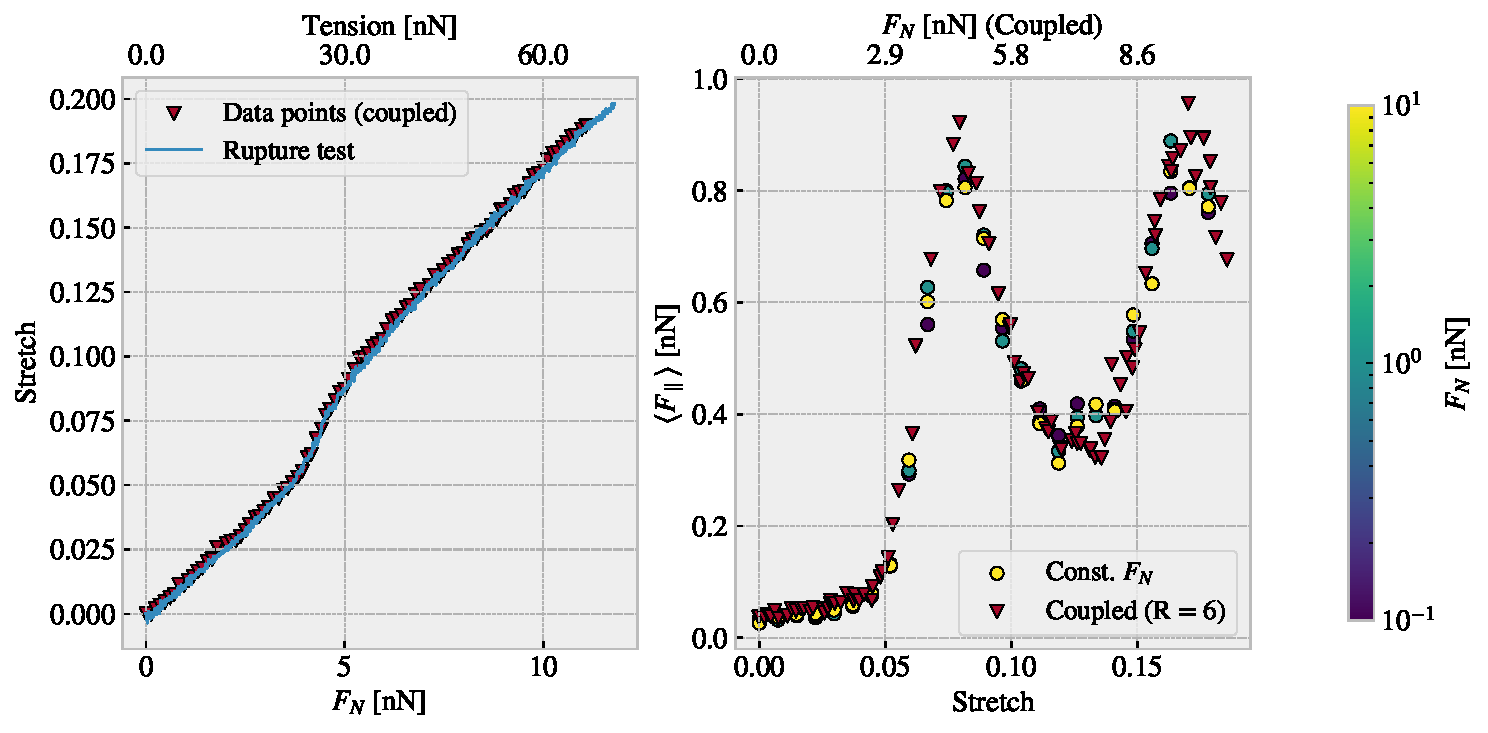
\includegraphics[width=0.9\linewidth]{figures/negative_coefficient/manual_coupling_free_pop1_7_5.pdf}
  \caption{\hl{Maybe swap top and lower x-axis for right figure}}
  \label{fig:nanomachine}
\end{figure}

\begin{figure}[H]
  \centering
  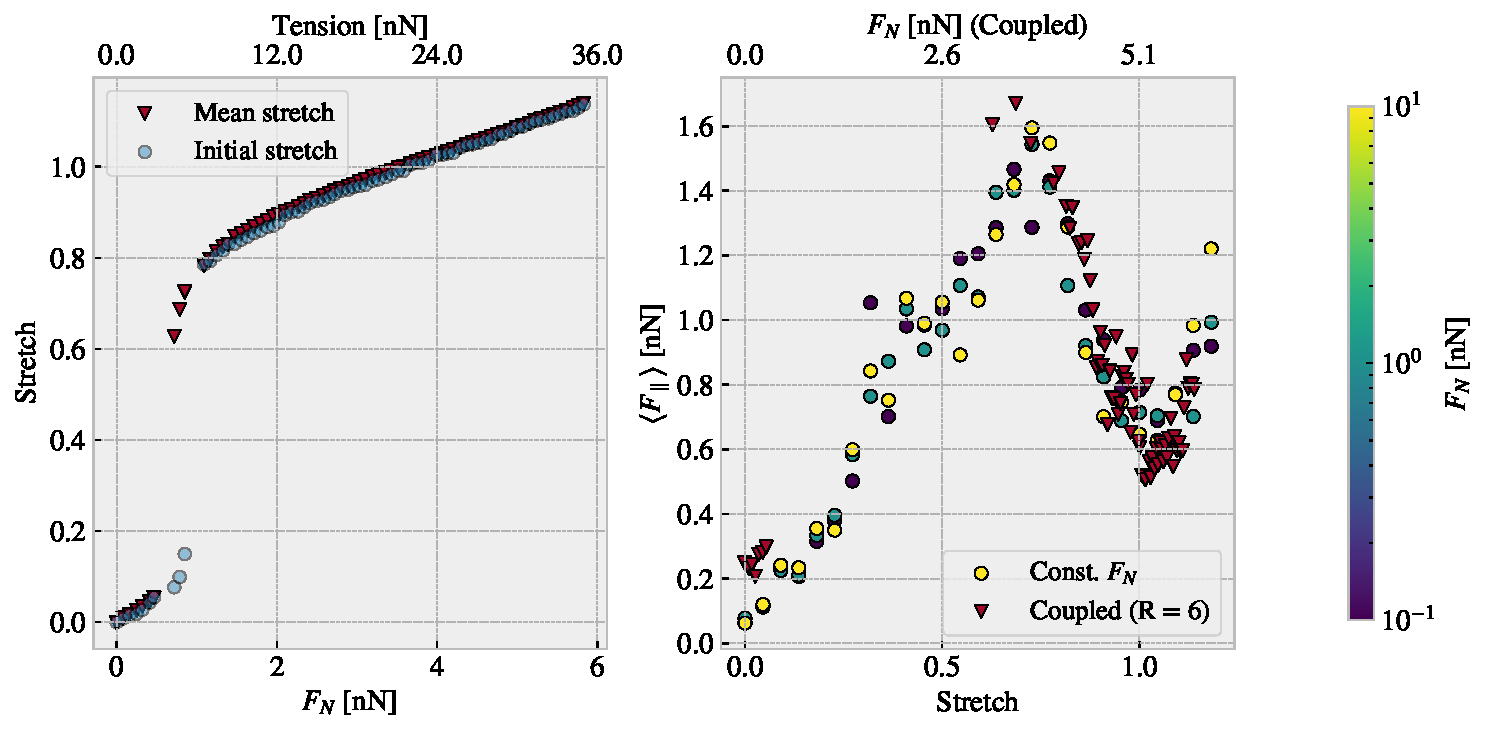
\includegraphics[width=0.9\linewidth]{figures/negative_coefficient/manual_coupling_free_hon3215.pdf}
  \caption{Fetch last data and update figure. Can we got more points in the sparse area?}
  \label{fig:nanomachine}
\end{figure}


For the honeycomb we had to lower the stretch speed (from 0.001 to 0.0001, explain what it means) due to the very abrupt change in the stretch tension curve. 


\section{Nanomachine coupling}
Attempt to couple normal force and stretch by crossed carbon nanotube (CNT) contraption \cref{fig:nanomachine}. 


\begin{figure}[H]
  \centering
  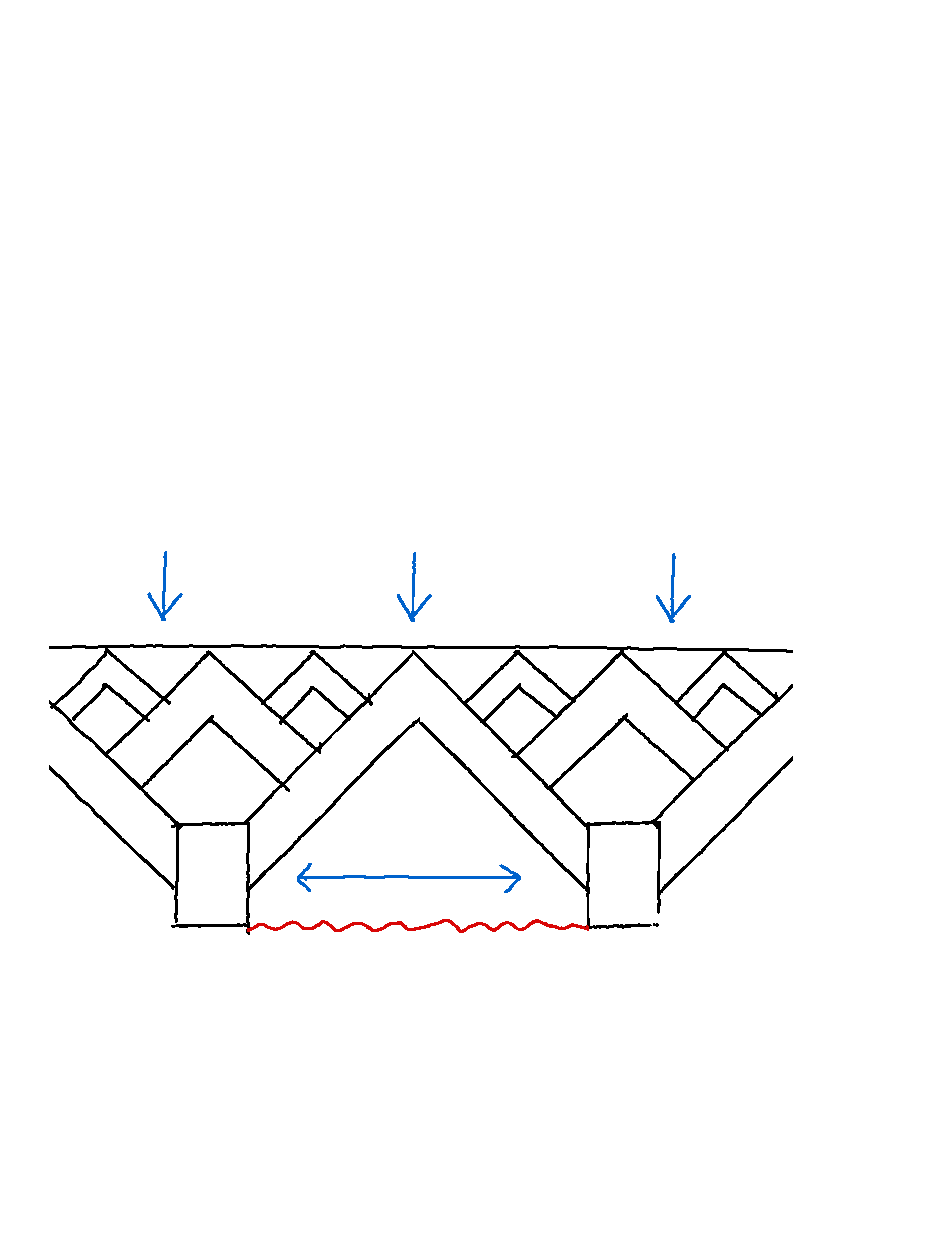
\includegraphics[width=0.5\linewidth]{figures/negative_coefficient/nanomachine.pdf}
  \caption{Working sketch for nanomachine}
  \label{fig:nanomachine}
\end{figure}



